\documentclass[10pt]{beamer}

\usepackage[utf8]{inputenc}
\usepackage[T1]{fontenc}
\usepackage[italian]{babel}
\usepackage{graphicx}
\usepackage{amsmath}
\usepackage{listings}
\usepackage{xcolor}

% --- Tema e Colori Beamer ---
\usetheme{metropolis}

% --- Configurazione per i blocchi di codice (listings) ---
\definecolor{codegreen}{rgb}{0,0.6,0}
\definecolor{codegray}{rgb}{0.5,0.5,0.5}
\definecolor{codepurple}{rgb}{0.58,0,0.82}
\definecolor{backcolour}{rgb}{0.98,0.98,0.98}

\lstdefinestyle{mystyle}{
    backgroundcolor=\color{backcolour},
    commentstyle=\color{codegreen},
    keywordstyle=\color{blue},
    stringstyle=\color{codepurple},
    basicstyle=\ttfamily\footnotesize,
    breakatwhitespace=false,
    breaklines=true,
    captionpos=b,
    keepspaces=true,
    showspaces=false,
    showstringspaces=false,
    showtabs=false,
    tabsize=2,
    frame=single,
    language=SQL
}
\lstset{style=mystyle}

\title{DietiEstates: Un Portale Immobiliare Moderno}
\subtitle{Presentazione del Progetto}
\author{Giorgio Di Fusco}
\institute{Università degli Studi di Napoli Federico II}
\date{\today}

\begin{document}

\begin{frame}
    \titlepage
\end{frame}

\begin{frame}{Agenda}
    \tableofcontents
\end{frame}

\section{Introduzione al Progetto}

\begin{frame}{Cos'è DietiEstates?}
    \begin{block}{Obiettivo del Progetto}
        \textbf{DietiEstates} è un portale immobiliare full-stack progettato per modernizzare l'interazione tra clienti, agenti immobiliari e gestori di agenzie.
        \vspace{1em}

        L'obiettivo è creare una piattaforma:
        \begin{itemize}
            \item \textbf{Performante:} Tempi di risposta rapidi e ricerca efficiente.
            \item \textbf{Intuitiva:} Esperienza utente pulita e facile da usare.
            \item \textbf{Sicura:} Autenticazione robusta e protezione dei dati.
            \item \textbf{Modulare:} Architettura manutenibile e scalabile.
        \end{itemize}
    \end{block}
\end{frame}

% ==================================================
\section{Utenti Target}
% ==================================================

\begin{frame}{Utenti del Sistema}
    Il sistema è stato modellato attorno a tre figure chiave:
    \begin{columns}[T]
        \begin{column}{.33\textwidth}
            \centering
            
\includegraphics[width=0.8\linewidth]{../res/lucia_moretti.jpg}
            \textbf{Lucia (Cliente)}
            \begin{itemize}
                \item Cerca casa in affitto.
                \item Frustrata da annunci vaghi e foto ingannevoli.
                \item Desidera una ricerca potente e dettagliata.
            \end{itemize}
        \end{column}
        \begin{column}{.33\textwidth}
            \centering
            
\includegraphics[width=0.8\linewidth]{../res/andrea_rinaldi.jpg}
            \textbf{Andrea (Agente)}
            \begin{itemize}
                \item Gestisce un portafoglio di immobili.
                \item Vuole inserire annunci dettagliati.
                \item Necessita di un sistema efficiente per gestire le visite.
            \end{itemize}
        \end{column}
        \begin{column}{.33\textwidth}
            \centering
            
\includegraphics[width=0.5\linewidth]{../res/marco_de_santis.jpg}
            \textbf{Marco (Gestore Agenzia)}
            \begin{itemize}
                \item Supervisiona l'agenzia.
                \item Necessita di strumenti per gestire i collaboratori.
            \end{itemize}
        \end{column}
    \end{columns}
\end{frame}

\section{Funzionalità Principali}

\begin{frame}{Casi d'Uso}
    \begin{figure}
        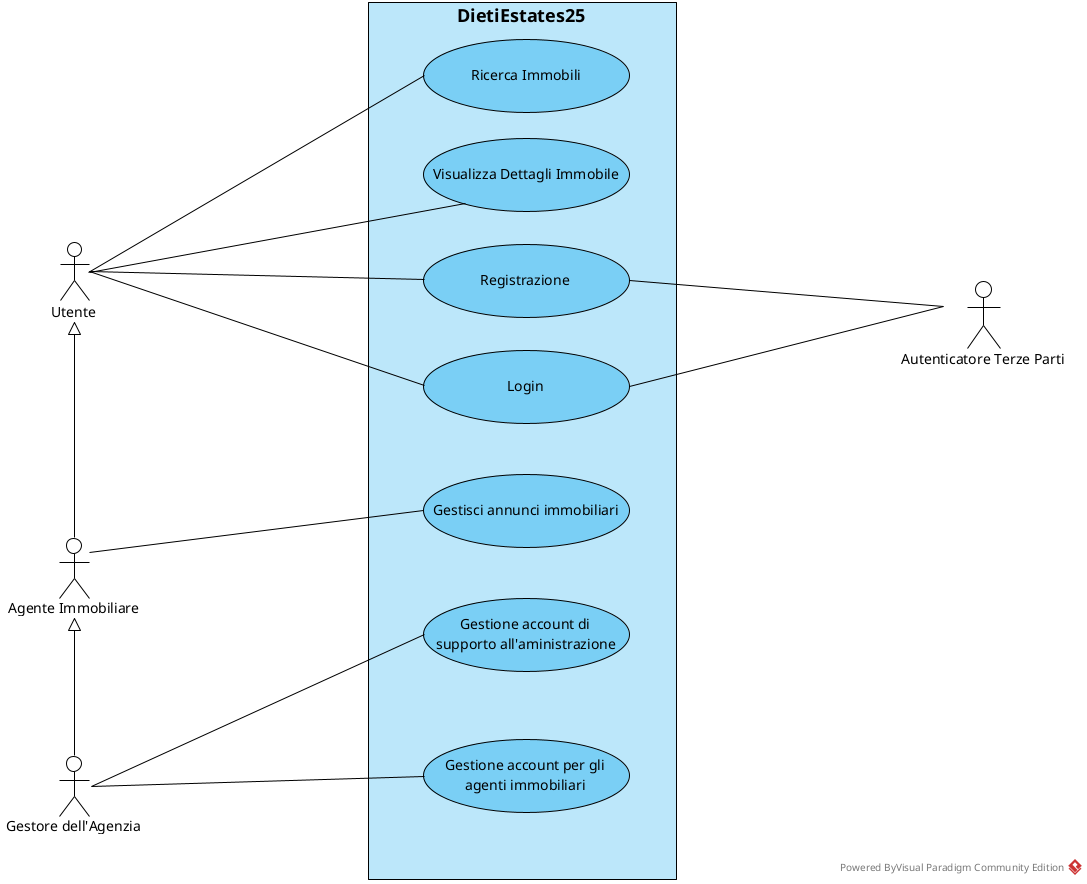
\includegraphics[width=0.8\textwidth]{../res/Use Case Diagram.png}
        \caption{Diagramma dei Casi d'Uso principali del sistema.}
    \end{figure}
\end{frame}

\begin{frame}{Funzionalità Chiave}
    \begin{block}{Per il Cliente}
        \begin{itemize}
            \item Ricerca base e avanzata su mappa interattiva.
            \item Visualizzazione dettagliata degli annunci.
            \item Gestione profilo.
        \end{itemize}
    \end{block}
    \begin{block}{Per l'Agente e il Gestore}
        \begin{itemize}
            \item \textbf{Gestione Annunci (CRUD):} Creazione, modifica e rimozione di inserzioni con gallerie di immagini.
            \item \textbf{Gestione Collaboratori:} Un gestore può aggiungere nuovi agenti e promuoverli a ruoli con maggiori privilegi (\texttt{ADMIN\_ASSISTANT}).
        \end{itemize}
    \end{block}
\end{frame}

\section{Architettura e Design}

\begin{frame}{Architettura del Sistema: Three-Tier}
    Il sistema segue un'architettura a tre livelli per garantire modularità e disaccoppiamento.
    \vspace{1em}

    \begin{block}{Presentation Tier (Frontend)}
        \begin{itemize}
            \item \textbf{Single-Page Application (SPA)} sviluppata in \textbf{Angular}.
            \item Responsabile dell'interfaccia utente e delle interazioni.
            \item Comunica con il backend tramite API REST.
        \end{itemize}
    \end{block}

    \begin{block}{Application Tier (Backend)}
        \begin{itemize}
            \item Applicazione \textbf{Spring Boot} che espone API RESTful.
            \item Implementa la logica di business, l'autenticazione e l'autorizzazione.
        \end{itemize}
    \end{block}

    \begin{block}{Data Tier (Database)}
        \begin{itemize}
            \item Database relazionale \textbf{PostgreSQL} per la persistenza dei dati.
            \item Accesso gestito tramite \textbf{Spring Data JPA} e Hibernate.
        \end{itemize}
    \end{block}
\end{frame}

\begin{frame}{Tecnologie Adottate}
    \begin{columns}[T]
        \begin{column}{.5\textwidth}
            \begin{block}{Backend}
                \begin{itemize}
                    \item \textbf{Java 17} e \textbf{Spring Boot}
                    \item \textbf{Spring Security} (JWT, OIDC)
                    \item \textbf{JPA / Hibernate}
                    \item \textbf{PostgreSQL + PostGIS}
                    \item \textbf{Maven}
                    \item \textbf{Docker}
                \end{itemize}
            \end{block}
        \end{column}
        \begin{column}{.5\textwidth}
            \begin{block}{Frontend}
                \begin{itemize}
                    \item \textbf{Angular} e \textbf{TypeScript}
                    \item \textbf{OpenAPI Generator}
                    \item HTML5 / CSS3 (Bootstrap)
                    \item Leaflet.js (Mappe)
                \end{itemize}
            \end{block}
        \end{column}
    \end{columns}
    \begin{block}{Integrazioni Esterne}
        \begin{itemize}
            \item \textbf{Amazon S3:} per lo storage di oggetti (immagini degli annunci).
            \item \textbf{Provider OIDC} (es. Google) per l'autenticazione esterna.
        \end{itemize}
    \end{block}
\end{frame}

\begin{frame}{Backend Design: Monolite Modulare (DDD)}
    \begin{block}{Approccio}
        Il backend è un \textbf{monolite modulare} strutturato secondo i principi del \textbf{Domain-Driven Design (DDD)}.
        \begin{itemize}
            \item Ogni package Java rappresenta un \textbf{Bounded Context} con responsabilità ben definite.
            \item Questo approccio favorisce la manutenibilità e la futura evoluzione verso microservizi.
        \end{itemize}
    \end{block}
    \begin{block}{Bounded Contexts Principali}
        \begin{itemize}
            \item \texttt{auth}: Gestione utenti, ruoli e autenticazione.
            \item \texttt{listings}: Cuore del dominio, gestione annunci immobiliari.
            \item \texttt{agency}: Logica per agenzie e gestione collaboratori.
            \item \texttt{file}: Servizio di supporto per lo storage su S3.
            \item \texttt{email}: Servizio di supporto per le notifiche.
            \item \texttt{security}: Infrastruttura per la sicurezza (JWT, filtri).
        \end{itemize}
    \end{block}
\end{frame}

% ==================================================
\section{Approfondimenti Tecnici}
% ==================================================

\begin{frame}[fragile]{Deep Dive: Ricerca Geospaziale con PostGIS}
    \begin{block}{Problema}
        Permettere agli utenti di cercare immobili entro un raggio specifico da un punto sulla mappa.
    \end{block}
    \begin{block}{Soluzione}
        \begin{itemize}
            \item Utilizzo dell'estensione \textbf{PostGIS} per PostgreSQL.
            \item Le coordinate degli immobili sono salvate in un campo di tipo \texttt{geometry(Point, 4326)}.
            \item Le query sfruttano indici spaziali (GIST) e funzioni native per calcoli geodetici efficienti.
        \end{itemize}
    \end{block}
    \begin{exampleblock}{Esempio di Query di ricerca per raggio}
\begin{lstlisting}[language=SQL]
SELECT l.* FROM listing l
WHERE ST_DWithin(
    l.coordinate::geography,
    ST_SetSRID(ST_MakePoint(:lon, :lat), 4326)::geography,
    :radius_meters
);
\end{lstlisting}
    \end{exampleblock}
\end{frame}

\begin{frame}{Deep Dive: Gestione della Sicurezza}
    \begin{block}{Autenticazione e Autorizzazione}
        La sicurezza è gestita da \textbf{Spring Security} con un approccio \textit{stateless}.
        \begin{itemize}
            \item \textbf{Autenticazione via Credenziali:} Generazione di \textbf{JWT Access Token} e \textbf{Refresh Token}.
            \item \textbf{Autenticazione via Provider Esterni:} Supporto a \textbf{OpenID Connect (OIDC)} (es. Google) tramite il pattern \textit{OAuth2UserInfoFactory}.
            \item \textbf{Autorizzazione:} Gestita tramite una \texttt{SecurityFilterChain} che protegge gli endpoint in base ai ruoli (\texttt{ADMIN}, \texttt{AGENT}, \texttt{USER}).
        \end{itemize}
    \end{block}                              
\end{frame}

\begin{frame}{Deep Dive: Gestione delle Immagini}
    \begin{block}{Separazione delle Responsabilità}
        Per garantire scalabilità e performance, i dati binari sono separati dai metadati.
        \begin{itemize}
            \item \textbf{Amazon S3:} Utilizzato come object storage per salvare i file delle immagini. È scalabile, robusto e ottimizzato per la distribuzione di contenuti.
            \item \textbf{PostgreSQL:} Memorizza solo i metadati associati alle immagini (URL, ordine di visualizzazione, riferimento all'annuncio).
        \end{itemize}
    \end{block}
    \begin{alertblock}{Vantaggi}
        \begin{itemize}
            \item Il database rimane leggero e performante.
            \item Lo storage degli asset può scalare indipendentemente.
            \item Si sfruttano le CDN e le feature di S3 per una consegna rapida delle immagini.
        \end{itemize}
    \end{alertblock}
\end{frame}

% ==================================================
\section{Conclusioni}
% ==================================================

\begin{frame}{Conclusioni e Sviluppi Futuri}
    \begin{block}{Risultati Raggiunti}
        \begin{itemize}
            \item Realizzazione di una piattaforma immobiliare completa e funzionale.
            \item Architettura solida, modulare e basata su tecnologie moderne.
            \item Implementazione di funzionalità complesse come la ricerca geospaziale e un sistema di sicurezza robusto.
        \end{itemize}
    \end{block}
    \begin{block}{Sviluppi Futuri}
        \begin{itemize}
            \item Completamento della gestione appuntamenti.
            \item Integrazione di un sistema di notifiche in-app.
            \item Dashboard analitiche avanzate per i gestori di agenzia.
            \item Evoluzione verso un'architettura a microservizi partendo dai Bounded Contexts già definiti.
        \end{itemize}
    \end{block}
\end{frame}

% --- DOMANDE ---
\begin{frame}
    \begin{center}
        \Huge{\textbf{Domande?}}
    \end{center}
\end{frame}

\end{document}
